% Created 2018-09-26 Wed 21:07
% Intended LaTeX compiler: pdflatex
\documentclass[journal=ancac3,manuscript=article,email=true,hyperref=true,keywords=false]{achemso}
\usepackage[utf8]{inputenc}
\usepackage{graphicx}
\usepackage{float}
\usepackage{xcolor}
\usepackage{amsmath}
\usepackage{amssymb}
\usepackage{lineno}
\usepackage{todonotes}
\usepackage{times}

%\usepackage{xr}
\usepackage{xr-hyper} 
\externaldocument[SI-]{SI}



\author{Tian Tian}
\affiliation{Institute for Chemical and Bioengineering, ETH Z{\"{u}}rich,  Vladimir Prelog Weg 1, CH-8093 Z{\"{u}}rich, Switzerland}
\altaffiliation{T. T. and D. S. contributed equally to this work}
\author{Declan Scullion}
\affiliation{School of Mathematics and Physics, Queen's University Belfast, BT7 1NN, United Kingdom}
\altaffiliation{T. T. and D. S. contributed equally to this work}
\author{Dale Hughes}
\affiliation{School of Mathematics and Physics, Queen's University Belfast, BT7 1NN, United Kingdom}
\author{Lu Hua Li}
\affiliation{Institute for Frontier Materials, Deakin University, Victoria, VIC 3216, Australia}
\author{Chih-Jen Shih}
\affiliation{Institute for Chemical and Bioengineering, ETH Z{\"{u}}rich,  Vladimir Prelog Weg 1, CH-8093 Z{\"{u}}rich, Switzerland}
\author{Jonathan Coleman}
\affiliation{School of Physics, Centre for Research on Adaptive Nanostructures and Nanodevices (CRANN) and Advanced Materials and BioEngineering Research (AMBER), Trinity College Dublin, Dublin 2, Ireland}
\author{Manish Chhowalla}
%% \affiliation{Materials Science and Engineering, Rutgers University, 607 Taylor Road, Piscataway, New Jersey 08854, USA.}
\affiliation{Department of Materials Science \& Metallurgy, University of Cambridge, CB3 0FS, United Kingdom}
\author{Elton J. G. Santos}
\email{e.santos@qub.ac.uk}
\affiliation{School of Mathematics and Physics, Queen's University Belfast, BT7 1NN, United Kingdom}
\date{}
\title{Electronic polarizability as the fundamental variable in the dielectric properties of two-dimensional materials}
%\title{The Unified Nature of the Dielectric Properties of Two-Dimensional Materials}
% \title{Unified Understanding of the Dielectric Nature of Two-Dimensional Materials}

\keywords{Dielectric screening, electronic polarizability, two-dimensional material, scaling relation, first principles simulations, dielectric anisotropy}

% \begin{tocentry}
 % \centering
% \includegraphics[width=0.70\linewidth]{img/toc_v121719.pdf}  %toc.pdf  
% \end{tocentry}
%
%
%  \includegraphics[width=0.70\linewidth]{img/fig1.pdf}


\begin{document}

\newpage{}


% \section{Introduction}
% \label{sec:org2ea169d}
\linenumbers{}

\begin{abstract}
  The dielectric constant, which defines the polarization of
  the media, is a key quantity in condensed matter. It determines 
  several electronic and optoelectronic properties important for a 
  plethora of modern technologies 
  from computer memory to field effect
  transistors and communication circuits. Moreover, the importance of
  the dielectric constant in 
  describing electromagnetic interactions through screening plays a
  critical role in understanding fundamental molecular
  interactions. Here we show that despite its fundamental
  transcendence, the dielectric constant does not define unequivocally
  the dielectric properties of two-dimensional (2D) materials due to
  the locality of their electrostatic screening. Instead, the
  electronic polarizability correctly captures the dielectric nature
  of a 2D material which is united to other physical quantities in an
  atomically thin layer. 
 %
  %
%  Being a quantity with unique definition, the
%  electronic polarizability overcomes the disadvantage of uncertainty
%  posed by the effective dielectric constant model conventionally used
%  to described screening in 2D material systems.  
  We reveal a long-sought universal formalism where electronic, 
  geometrical and dielectric properties are intrinsically correlated  
  through the polarizability opening the door to probe quantities yet  
  not directly measurable including the real covalent thickness of a 
  layer. We unify the concept of dielectric properties in any 
  material dimension finding a global dielectric anisotropy index
  defining their controllability through dimensionality. 
\end{abstract}

\pagebreak{}

\section{Introduction}
\label{sec:introduction}

The dielectric constant $\varepsilon$ (also known as the relative permittivity) 
plays a crucial role in bridging various fundamental material
properties, such as bandgap \cite{Moss_1950_relation,Moss_1985_n_Eg}, 
optical absorption\cite{kittel_2005_introduction} and 
conductivity \cite{Dressel_2001_electrodynamics}   
with elemental interactions. 
The central place of $\varepsilon$ in solid-state physics drives the analysis of several phenomena 
where is common to classify a material accordingly to its ability to screen an 
electric field $\boldsymbol{E}$ in terms of insulators, metals and semiconductors. 
Such definitions determine a broad range of 
condensed matter physics, as well as in related 
fields in chemistry and materials science. 
The ability to compute and measure $\varepsilon$ in 
bulk materials is well established via different 
theoretical \cite{Adler_1962,Hybertsen_1987} and 
experimental techniques \cite{palik_1998handbook} of distinct flavors
where the probe of the dielectric properties 
is made through an external electric field. 
%
Despite its obvious appeal, however, it is 
still unknown whether such quantity can determine the 
electronic and dielectric properties of 
two-dimensional (2D) materials \cite{Novoselov_2016}.  
%
The confined nature of such atomically-thin 2D crystals associated
with the attenuated and anisotropic character of the dielectric
screening
\cite{Keldysh_1979_eps_multi,Sharma_1985,Low_2014_screening_BP,Cudazzo_2011_screening_2D,Bechstedt_2012,Cudazzo_2010_screen2D,Nazarov_2015_2D_3D}
has generated long-standing debates whether the dielectric constant
truly represents the dielectric features of such low-dimensional systems. 
%or it can be used only as an
%additional parameter from the bulk-counterparts.
%
%
The controversy of values
reported by both theoretical and experimental
approaches can be widely seen throughout the specialized 
literature, see Ref.\cite{Li_2016} for a summary,
where the variation of $\varepsilon$ can be more than one order of
magnitude. As a consequence, several key physical parameters that
scale with $\varepsilon$, such as the exciton binding energy and
Debye screening length, cannot be reliably estimated due to the
discrepancy of the reported magnitudes of $\varepsilon$. 

Here, by using a combination of analytical and numerical models liaised with 
highly-accurate first-principles methods involving high-throughput screening 
techniques, we show that the dielectric constant does not provide a reliable
description of the screening features of a 2D material. The interplay between local 
electrostatic interactions in the monolayer and the volume dependence 
in the definition of $\varepsilon$ makes such quantity questionable. 
%
%
We propose however that the electronic polarizability that describes 
the electron dipole in the 2D material as the true descriptor 
of its dielectric nature. 
%
%
We overcome several problems intrinsic to thin layers not achievable using conventional 
effective dielectric medium models, such as the real thickness of a monolayer and 
any dependence on the long-range Coulomb potential. 
We unveil universal scaling relations between electronic and dielectric properties through 
the electronic polarizability, such as band gaps, optical spectra and exciton radius, for the 
current library of known 2D materials involving different lattice symmetries, 
atomic elements and chemical and physical properties. 
%
Moreover, the concept of electronic polarizabilities bridges the
gap between the dielectric properties of 2D and 3D systems through a novel 
dielectric anisotropy index that generalized the concept of dielectric control 
using dimensionality and bandgap. 
Our results open a new avenue for the study of the 
dielectric properties of 2D compounds using techniques yet to be explored. 


%and can be
%extended to characterize the dielectric anisotropy for any material
%dimensions.


%%
%%

\section{Results and discussions}
\label{sec:results-discussions}

\subsection{Lattice-dependency of macroscopic dielectric constant}
\label{sec:latt-depend-macr}

We first approach the discrepancy of macroscopic dielectric constant
of 2D materials, by showing that the current definition of
$\varepsilon$ used in layered materials is {ill-defined}.  This can be
viewed in a model system as illustrated
in Figure \ref{fig-1}, where an isolated 2D material is placed in
the \textit{xy}-plane of a periodically repeating superlattice (SL)
with a length $L$ along the \textit{z}-direction separating the cell
images. The static macroscopic dielectric tensor from the superlattice
$\varepsilon_{\mathrm{SL}}^{pq}$, is determined through fundamental
electrostatics by the response of the polarization density
$\boldsymbol{P}^{p}$ under small perturbative external field
$\boldsymbol{E}^{q}$, where $p$, $q$ determine their directions,
respectively~\cite{Dressel_2001_electrodynamics}:
\begin{subequations}
  \begin{eqnarray}
      \label{eq:def-eps-1}
    &\varepsilon_{\mathrm{SL}}^{pq} &= \kappa^{pq} +
                                 {\displaystyle \frac{\partial \boldsymbol{P}^{p}}{\varepsilon_{0} \partial \boldsymbol{E}^{q}}} \\
          \label{eq:def-eps-2}
    &\boldsymbol{P}^{p} &=  {\displaystyle \frac{\boldsymbol{u}^{p}}{\Omega}}
                          = {\displaystyle \frac{{\displaystyle
          \int_{\mathrm{SL}} \rho(\boldsymbol{r}) \boldsymbol{r}^{p} d^{3}\boldsymbol{r}}}{AL}}
  \end{eqnarray}
\end{subequations}
where $\kappa$ is the dielectric tensor of the environment,
$\boldsymbol{u}$ is the total dipole moment within the SL, $\rho$ is
the spatial charge density, $\Omega=AL$ is the volume of the
supercell, $A$ is the \textit{xy}-plane area of the SL and
$\varepsilon_{0}$ is vacuum permittivity. Here we limit our study on
the electronic contributions to the macroscopic dielectric constant
where the dipole $\boldsymbol{P}$ results from the response 
of the electron density under an external field.  
Ionic contributions\cite{Sohier_2017} to $\varepsilon_{\mathrm{SL}}$ 
have previously been shown to be negligible\cite{relax-epsilon} and 
are not considered here.  
%
%On the other hand, the ionic
%contribution to $\varepsilon_{\mathrm{SL}}$ that comes from
%displacement of atomic nuclei is not covered in this due to its
%complex dependency on several factors including phonon
%dispersion~\cite{Sohier_2017} as well as lattice
%symmetry~\cite{Laturia_2018}, which requires separated discussions.
The symmetry of 2D materials leads to inappreciable off-diagonal
elements of the dielectric tensor ($p \neq q$), while the diagonal
elements $\varepsilon_{\mathrm{SL}}^{xx}$,
$\varepsilon_{\mathrm{SL}}^{yy}$ and $\varepsilon_{\mathrm{SL}}^{zz}$
can be different \cite{Sohier_2016}.  
%
Considering that the 2D material
is placed in vacuum ($\kappa^{pp} = 1$ and $\kappa^{pq} = 0$), we can
distinguish two components of $\varepsilon_{\mathrm{SL}}$, namely the
in-plane ($\varepsilon_{\mathrm{SL}}^{\parallel}$) and out-of-plane
($\varepsilon_{\mathrm{SL}}^{\perp}$) dielectric constants, where
$\varepsilon_{\mathrm{SL}}^{\parallel} =
(\varepsilon_{\mathrm{SL}}^{xx} + \varepsilon_{\mathrm{SL}}^{yy})/2$
and
$\varepsilon_{\mathrm{SL}}^{\perp} = \varepsilon_{\mathrm{SL}}^{zz}$.
The absence of bonding perpendicular to the plane confines the induced
dipole moments along the \textit{z}-direction within a range of $\sim$5--6
\AA{} into the vacuum (Figure \ref{fig-1}{\textbf a} and Supplementary
Figure \ref{SI-fig:rho-profile}).
%
%
Under a given external field, the strong confinement of
the induced dipole moment $\boldsymbol{u}$ causes the integral in the 
numerator of Eq.~\ref{eq:def-eps-2} to be converged within few \AA's 
resulting that the dipole moment from the periodic supercell 
images do not mutually interfere. 
%


Conversely, the increase of
$L$ in the denominator of Eq.~\ref{eq:def-eps-2} dilutes the 
polarization density, and in turn makes both
$\varepsilon^{\parallel}_{\mathrm{SL}}$ and
$\varepsilon^{\perp}_{\mathrm{SL}}$ dropping to
unity when $L$ is infinitely large, which is not physical. 
% In the case of bulk materials
% such physical dependence is well described given the periodicity of
% the 3D crystal throughout the space.
%
%since this volume is used to represent the crystal 
%periodically throughout the space.  
%
%
% In the case of 2D materials, however, such repetition is artificial along the direction 
% perpendicular to the plane.
Despite the simplicity of this argument, any calculation performed
using such definition will intrinsically depend on the magnitude of
$L$, an artificial parameter introduced by the simulation setup. This
dependence can be clearly demonstrated by plotting
$\varepsilon^{\parallel}_{\mathrm{SL}}$ and
$\varepsilon^{\perp}_{\mathrm{SL}}$ calculated from density functional
theory (DFT) (see {\it Theoretical Methods} for details) as a function
of $L$ for P\={6}m2 transition metal dichalcogenides (TMDCs),
2H-MX$_{2}$, where M=Mo, W and X=S, Se, Te (top panels of Figure
\ref{fig-1}{\textbf b} and \ref{fig-1}{\textbf c}, respectively). To
obtain a better description of the electronic band structure, the
calculations of dielectric properties were performed at the level of
Heyd-Scuseria-Ernzerhof (HSE06) hybrid functional
\cite{Heyd_2003,HSE_2006}.  Both components of the dielectric
constant decrease with $L$ as excepted. To rule out the possibility
that the result is affected by the choice of the functional, 
we performed simulations at higher levels of theory
using many-body techniques (G$_{0}$W$_{0}$), which invariably give
alike results (see Supplementary Figure \ref{SI-fig:GW-PBE-alpha}).
The lattice-size dependency also exists for the dielectric function in the 
frequency domain. 

\begin{figure}[H]
\centering
\includegraphics[width=0.70\linewidth]{img/fig1.pdf}
\caption{\label{fig-1} \textbf{2D polarizability and the breakdown of
    effective dielectric model
    (EDM)} % \textbf{2D polarizability as the
  % true descriptor of the dielectric nature of 2D materials.}
  \textbf{a,} 3D illustration of the spatial distribution of the
  charge density change $\Delta \rho(z)$ along the z-direction for
  monolayer 2H-MoS\textsubscript{2} in a periodic superlattice under
  external eletric field of 0.01 V/\AA{}.  The green and red regions
  represent negative and positive induced charges, respectively. The
  macroscopic $\varepsilon_{\mathrm{SL}}^{\parallel}$ and
  $\varepsilon_{\mathrm{SL}}^{\perp}$ are influenced by the lattice
  size $L$, while the 2D polarizabilities
  $\alpha_{\mathrm{2D}}^{\parallel}$ and
  $\alpha_{\mathrm{2D}}^{\perp}$ are invariant to $L$.
  \textbf{b,} $\varepsilon^{\parallel}_{\mathrm{SL}}$ (top) and
  $\alpha_{\mathrm{2D}}^{\parallel}$ (bottom) as functions of $L$ for
  the 2H TMDCs. 
  \textbf{c,} $\varepsilon^{\perp}_{\mathrm{SL}}$ (top)
  and $\alpha_{\mathrm{2D}}^{\perp}$ (bottom) as functions of $L$ for
  the 2H TMDCs. The polarizabilities in \textbf{b} and \textbf{c} are
  constant when $L>$15 \AA{}, compared with the $L$-dependence of
  $\varepsilon_{\mathrm{SL}}$. 
  %
  %
  {\bf d-e,} Estimated $\varepsilon_{\mathrm{2D}}^{\parallel}$ and 
  $\varepsilon_{\mathrm{2D}}^{\perp}$, respectively, using EDM  
  as a function of the uncertainty of the effective layer
  thickness $\delta^{*}_{\mathrm{2D}}$. The inset in {\bf e,} shows schematically the main parameters
  utilized in EMD: the vacuum layer ($\varepsilon^{}_{\mathrm{0}}$), an approximate thickness of the layer   which is given by $\delta^{*}_{\mathrm{2D}}$, and the obtained $\varepsilon^{}_{\mathrm{2D}}$. The length of the box perpendicular to the surface of the layer is given by $L$ (not shown). 
  %
  Overall, there is a large variation and associated errors
  to both components of the dielectric constant for small changes of $\delta^{*}_{\mathrm{2D}}$ in the range of $\pm7.5$\%.  
  %
  % HSE06 functional is used in all plots.
}
\end{figure}


We carried out similar analysis for
frequency-dependent $\varepsilon^{\parallel}_{\mathrm{SL}}(\omega)$
and $\varepsilon^{\perp}_{\mathrm{SL}}(\omega)$ using different 
approaches including Perdew-Burke-Ernzerhof (PBE)
exchange-correlation functional
\cite{Perdew_1996,Ernzerhof99,Paier_2005_PBE}, 
G\textsubscript{0}W\textsubscript{0}\cite{Hedin_1965} and
Bethe-Salpeter equation (G\textsubscript{0}W\textsubscript{0}$-$BSE)\cite{Onida_2002} (see Supplementary Section \ref{SI-ssec:gw} and 
Supplementary Figures \ref{SI-fig:PBE-omega-in}$-$\ref{SI-fig:BSE-omega-out}). 
%
%with increasing
%accuracy of calculated optical properties (PBE $<$
%G\textsubscript{0}W\textsubscript{0} $<$ BSE) due to including of
%many-body screening and excitonic effects (details see Supplementary
%Section \ref{SI-ssec:gw}). 
%
Despite the various levels of theory analyzed and the increased 
accuracy of the calculated optical properties due to the inclusion of 
many-body screening and excitonic effects, 
the magnitude of the dielectric function universally decreases
with $L$ over the frequency. The underlying physical reason for such 
dependence can be noticed in the definition of the dielectric 
function versus $\omega$ shown in Eqs. \ref{SI-eq:dft-dielectric}$-$\ref{SI-eq:dft-dielectric-real}, which also depend on the volume of the unit cell. 
%
These results indicate that any 
quantity that depends on
$\varepsilon^{\parallel}_{\mathrm{SL}}(\omega)$ and
$\varepsilon^{\perp}_{\mathrm{SL}}(\omega)$, such as the optical
absorption ($\mathrm{Im}\{\varepsilon_{\mathrm{SL}}(\omega)\}$), refractive index ($n=\sqrt{\mathrm{Re}\{\varepsilon_{\mathrm{SL}}\}}$) and electron energy loss spectrum (EELS, $\mathrm{Im}\{-1/\varepsilon_{\mathrm{SL}}(\omega)\}$), suffers the same deficiencies for 2D materials. 



\subsection{The electronic polarizability of 2D materials}
\label{sec:electr-polar-2d}

To solve the problem described above, we need to find the
$L$-independent alternative of $\varepsilon_{\mathrm{SL}}$, which is
related to both electrostatic and optical properties of a 2D
material~\cite{Matthes_2016}. By multiplying Eq.~\ref{eq:def-eps-2}
with $L$, we obtain the sheet polarization density, that is,
$\boldsymbol{\mu}_{\mathrm{2D}}^{p} =\boldsymbol{u}^{p}/A$, along the
direction $p$. Following the discussion in the previous section,
$\boldsymbol{\mu}_{\mathrm{2D}}^{p}$ becomes independent of the
lattice size when $L$ is large enough, due to the short decay of the 
induced charge density $\Delta \rho$ into the vacuum (see
Supplementary Figure \ref{SI-fig:rho-profile}).
%
Similar to the molecular polarizability\cite{Israelachvili_2011}, we
utilize the concept of electronic polarizability
$\alpha_{\mathrm{2D}}$, 
which has been used previously to solve
exciton-related problems in 2D materials
\cite{Cudazzo_2011_screening_2D,Olsen_2016_hydrogen,Jiang_2017_Eg_Eb}. 
%
$\alpha_{\mathrm{2D}}$ is a macroscopic quantity that characterizes
the ability to induce dipole moments in a 2D material, and is
associated with $\boldsymbol{\mu}_{\mathrm{2D}}$ through:
$\boldsymbol{\mu}_{\mathrm{2D}}^{p} = \sum_{q}
\alpha_{\mathrm{2D}}^{pq} \boldsymbol{\overline{E}}_{\mathrm{loc}}^{q}$\cite{T_bik_2004}, where
$\boldsymbol{\overline{E}}_{\mathrm{loc}}$ is the cell-averaged
``local'' electric field acting on the 2D material to induce
polarization\cite{}.
% 
Alike to $\mu_{\mathrm{2D}}$,
$\boldsymbol{\overline{E}}_{\mathrm{loc}}$ is also a macroscopic
quantity that excludes the fields generated by the dipoles of the 2D
sheet from $\boldsymbol{E}$. Note the term ``local'' in
$\boldsymbol{\overline{E}}_{\mathrm{loc}}$ is adapted to resemble the
Lorentz model\cite{Wiser_1963} which has also been used for other
low-dimensional materials (e.g. nanotube\cite{Benedict_1995} and
molecules\cite{T_bik_2004}, and should be distinguished with the
microscopic local field $\boldsymbol{E}_{\mathrm{loc}}(\boldsymbol{r})$ which is spatially
changing.
%


Such macroscopic treatment of polarizability is valid when the length
of the superlattice is significantly larger than the spatial
distribution of induced charges.  At $L \rightarrow \infty$ limit,
$\boldsymbol{\overline{E}}_{\mathrm{loc}}$ can be solved using
electrostatic boundary conditions of the slab geometry
\cite{Markel_2016,Meyer_2001_dipole_slab}. The continuity of the electric field along the
in-plane direction gives
$\boldsymbol{\overline{E}}^{\parallel}_{\mathrm{loc}}=\boldsymbol{E}^{\parallel}$,
while for the out-of-plane component, the dipole screening yields
$\boldsymbol{\overline{E}}_{\mathrm{loc}}^{\perp}=\boldsymbol{E}^{\perp}+\boldsymbol{\mu}_{\mathrm{2D}}^{\perp}/L$
\cite{Meyer_2001_dipole_slab,T_bik_2004}, where
$\boldsymbol{E}^{\parallel}$ and $\boldsymbol{E}^{\perp}$ are the
external field along the in-plane and out-of-plane directions,
respectively. Combining with Eqs. \ref{eq:def-eps-1} and
\ref{eq:def-eps-2}, $\alpha_{\mathrm{2D}}^{\parallel}$ and
$\alpha_{\mathrm{2D}}^{\perp}$ can be related with
$\varepsilon_{\mathrm{SL}}^{\parallel}$ and
$\varepsilon_{\mathrm{SL}}^{\perp}$, respectively:
%
%
\begin{subequations}
\begin{eqnarray}
  \label{eq:alpha-para-def}
  &\varepsilon_{\mathrm{SL}}^{\parallel} &= 1 + \frac{\alpha_{\mathrm{2D}}^{\parallel}}{\varepsilon_{0}L}\\
  \label{eq:alpha-perp-def}
  &\varepsilon_{\mathrm{SL}}^{\perp} &= \left(1 - {\displaystyle \frac{\alpha_{\mathrm{2D}}^{\perp}}{\varepsilon_{\mathrm{0}} L}} \right)^{-1}
\end{eqnarray}
\end{subequations}
% 20191003-16:00
% As pointed before, as we limit the discussion on electronic contributions to the dielectric properties, $\alpha_{\mathrm{2D}}$ characterizes the polarizability of electron cloud of a 2D materials.
% refers to the electronic polarizability (the polarizability of the
% electron cloud \cite{Israelachvili_2011}).

%
%
Using these relations, we show that the calculated
$\alpha_{\mathrm{2D}}^{\parallel}$ and $\alpha_{\mathrm{2D}}^{\perp}$
of the selected TMDCs as a function of $L$ in the bottom panels of
Figure \ref{fig-1}b and \ref{fig-1}c, respectively.  In contrast to
$\varepsilon_{\mathrm{SL}}^{\parallel}$ and
$\varepsilon_{\mathrm{SL}}^{\perp}$, we observe that both
$\alpha_{\mathrm{2D}}^{\parallel}$ and $\alpha_{\mathrm{2D}}^{\perp}$
reach convergence when $L \sim$10 \AA $, ~$15 \AA,
respectively. Such results are in good agreement with the spatially
localized induced dipole moment of a 2D material as shown in
Supplementary Figure~\ref{SI-fig:rho-profile}.
%
%
% Interestingly, we can use Eqs.\ref{eq:alpha-para-def} and
% \ref{eq:alpha-perp-def} to reproduce the trends noticed in the top
% panels in Figure\ref{fig-1}{\textbf b} and \ref{fig-1}{\textbf c} for
% $\varepsilon_{\mathrm{SL}}^{\parallel}$ and
% $\varepsilon_{\mathrm{SL}}^{\perp}$ as a function of $L$ around a
% centered magnitude of $\alpha_{\mathrm{2D}}^{\parallel}$ and
% $\alpha_{\mathrm{2D}}^{\perp}$
% (Figure \ref{fig-1}\textbf{d}-\textbf{e}).
% A similar curve profile is obtained in both components of the dielectric constant including the much 
% abrupt variation of $\varepsilon_{\mathrm{SL}}^{\perp}$ with $L$ which is due to 
% interlayer interactions.
%\todo[inline]{The original claim of this sentence, that $\varepsilon_{\mathrm{SL}}^{\perp}$ varies more due to interlayer interactions is not 100\% true. I think it is better not to explicitly mention this.}
Equations \ref{eq:alpha-para-def}$-$\ref{eq:alpha-perp-def} can 
also be used to remove the dependence on $L$ for
$\varepsilon^{\parallel}_{\mathrm{SL}}(\omega)$
and $\varepsilon^{\perp}_{\mathrm{SL}}(\omega)$, generating
lattice-independent electronic polarizability
$\alpha^{\parallel}_{\mathrm{SL}}(\omega)$ and
$\alpha^{\perp}_{\mathrm{SL}}(\omega)$ in the frequency domain,
respectively (see details in Supplementary Section \ref{SI-ssec:gw}).
%
% 
% 
% 
% 
These findings indicate that the electronic polarizability $\alpha_{\mathrm{2D}}$ captures the essence
of the dielectric properties of 2D materials. In contrast to the ill-defined macroscopic $\varepsilon_{\mathrm{SL}}$, $\alpha_{\mathrm{2D}}$ has 
a unique definition, and does not suffer from the dependency on the lattice size.
It is worthy mentioning that Eqs.\ref{eq:alpha-para-def}$-$\ref{eq:alpha-perp-def} were 
obtained using purely electrostatic arguments without any assumption 
regarding the medium where the 2D material is immersed or a capacitance 
model where an effective dielectric response can be extracted. 
More details about the choice of the
2D polarizability, comparison with other methods, simulations at the
frequency-dependent domain can be found in Supplementary Section
\ref{SI-ssec:gw}.




\subsection{Comparison with the effective dielectric model (EDM)}
\label{sec:comp-with-effect}

Apart from the 2D electronic polarizability proposed here,  
the effective dielectric model (EDM) is commonly used in
literature to treat the 2D material as a slab with an effective
dielectric tensor $\varepsilon_{\mathrm{2D}}$ and thickness
$\delta^{*}_{\mathrm{2D}}$. Such method can be found in both
experimental and theoretical studies, such as to interpret
ellipsometry data
\cite{graphene-epsilon10,Duesberg14,Chiang13,Kong14}, reflectance /
transmission spectra \cite{Li_2014, Yoffe-Wilson69}, optical
conductance \cite{Matthes_2016} and many-body interactions
\cite{Sohier_2016,Meckbach_2018} of 2D materials. The EDM allows
applying physical concepts of bulk systems directly to their 2D counterparts using
$\varepsilon_{\mathrm{2D}}$. However, there are several drawbacks of
such approach. For instance, the wavevector $q$-dependency of
dielectric screening in 2D
sheets~\cite{Cudazzo_2011_screening_2D,Olsen_2016_hydrogen,Trolle_2017_eps_subst}
is not captured. More severely, here we show that, due to the
uncertainty of $\delta^{*}_{\mathrm{2D}}$, the calculated
$\varepsilon_{\mathrm{2D}}$, in particular its out-of-plane component,
is extremely sensitive to the choice of $\delta^{*}_{\mathrm{2D}}$,
making such model questionable.

The basic assumption of EDM can be
seen in the inset of Figure~\ref{fig-1}\textbf{e}, where the macroscopic
$\varepsilon_{\mathrm{SL}}$ is considered to be composed by ({\it i}) a
2D slab with an effective dielectric constant $\varepsilon_{\mathrm{2D}}$
and a thickness $\delta^{*}_{\mathrm{2D}}$, and ({\it ii}) a vacuum spacing with
distance $L-\delta^{*}_{\mathrm{2D}}$. Using the effective medium theory
(EMT)~\cite{Aspnes_1982,Markel_2016}, the relation between  %Tancogne_Dejean_2015 
$\varepsilon_{\mathrm{SL}}$ and $\varepsilon_{\mathrm{2D}}$ can be
expressed using capacitance-like
equations~\cite{Matthes_2016,Laturia_2018,Tancogne_Dejean_2015}:
\begin{subequations}
  \begin{eqnarray}
    \label{Response:1}
    {\displaystyle \varepsilon_{\mathrm{SL}}^{\parallel}} &= {\displaystyle \frac{\delta^{*}_{\mathrm{2D}}}{L} \varepsilon_{\mathrm{2D}}^{\parallel} + \left(1 - \frac{\delta^{*}_{\mathrm{2D}}}{L} \right)}\\
     \label{eq:emt-2}
    {\displaystyle \frac{1}{\varepsilon_{\mathrm{SL}}^{\perp}}} &= {\displaystyle \frac{\delta^{*}_{\mathrm{2D}}}{L} \frac{1}{\varepsilon_{\mathrm{2D}}^{\perp}} + \left(1 - \frac{\delta^{*}_{\mathrm{2D}}}{L} \right)}
  \end{eqnarray}
\end{subequations}
In principle, both the values of $\varepsilon_{\mathrm{2D}}$ and
$\delta^{*}_{\mathrm{2D}}$ are unknown for a certain 2D material. To
minimize the modeling error, we used non-linear least-square fitting
to extract $\varepsilon_{\mathrm{2D}}$ and $\delta^{*}_{\mathrm{2D}}$ of
selected 2H TMDCs simultaneously from \textit{ab initio}
$\varepsilon_{\mathrm{SL}}$ -- $L$ data in
Figure~\ref{fig-1}\textbf{b} and \ref{fig-1}\textbf{c} (see details in 
Supplementary Figure~\ref{SI-fig:rescale-prb}). The fitted values of
the slab thickness, $\delta_{\mathrm{2D}}^{\parallel, \mathrm{fit}}$
and $\delta_{\mathrm{2D}}^{\perp, \mathrm{fit}}$ from in-plane and
out-of-plane data, respectively, are shown in Supplementary
Table~\ref{SI-tab:delta-L-DFt}.
%
% As seen in Figure
% \ref{fig-emt}\textbf{b}, the estimation error of the thickness
% estimated from different directions is around 0.06$\sim{}$0.27
% \AA{}.
%
Although the uncertainty only corresponds to a few percent of the
interlayer spacing in the bulk structure of these 2D materials, its
influence on the calculated values
$\varepsilon_{\mathrm{2D}}^{\parallel}$ and
$\varepsilon_{\mathrm{2D}}^{\perp}$ is substantial. 
We estimated the dispersion of $\varepsilon_{\mathrm{2D}}^{\parallel}$ and 
$\varepsilon_{\mathrm{2D}}^{\perp}$ considering slightly deviations of 
$\delta^{*}_{\mathrm{2D}}$ from the best fitted value by $\pm{}$7.5\%{} 
(Figures \ref{fig-1}\textbf{d} and \ref{fig-1}\textbf{e}). 
%
%
Strikingly, $\varepsilon_{\mathrm{2D}}^{\parallel}$ decays linearly
with $\delta^{*}_{\mathrm{2D}}$, while $\varepsilon_{\mathrm{2D}}^{\perp}$ spans
over more than one order of magnitude. 
%
The sensitivity of
$\varepsilon_{\mathrm{2D}}^{\perp}$ to $\delta^{*}_{\mathrm{2D}}$
explains the discrepancy in literature for both
isotropic~\cite{Sohier_2016} and highly
anisotropic~\cite{Matthes_2016,Laturia_2018}
$\varepsilon_{\mathrm{2D}}$ tensors on 2D materials extracted 
using EDM. 
%
As a consequence, the estimated values of
$\varepsilon_{\mathrm{2D}}$, in particular its out-of-plane component,
are highly controversial.

On the contrary, the proposed $\alpha_{\mathrm{2D}}$ approach does not
suffer from such limitations, despite its relatively simple
formalism. The relative uncertainty of $\alpha_{\mathrm{2D}}$ is
generally at the order of 10\textsuperscript{-4} (Supplementary
Figure~\ref{SI-fig:alpha-converg}). In addition, the calculation of
$\alpha_{\mathrm{2D}}$ is technically simpler than 
$\varepsilon_{\mathrm{2D}}$: ({\it i}) $\alpha_{\mathrm{2D}}$ can be
achieved using single-point calculation of macroscopic dielectric
tensor, while $\varepsilon_{\mathrm{2D}}$ requires non-linear fitting
of multiple $\varepsilon_{\mathrm{SL}}$ -- $L$ data points; ({\it ii}) the
values of $\alpha_{\mathrm{2D}}$ typically converge well for $L$
($\sim$20 \AA{}), while $\varepsilon_{\mathrm{2D}}$ suffers from the
uncertainties as described above.

%\subsection*{Polarizability as the fundamental variable}
%\label{sec:first-principles}

%We consider 

\subsection{Universal scaling laws of $\alpha_{\mathrm{2D}}$}
\label{sec:univ-scal-laws}

For bulk materials, pioneering works from the 1950s had demonstrated
empirical equations between $\varepsilon$ and the bandgap
$E_{\mathrm{g}}$, including the
Moss~\cite{Moss_1950_relation,Moss_1985_n_Eg,Finkenrath_1988} or
Ravindra~\cite{Ravindra_1980_model,Ravindra_1979_eps_Eg} relations.
Such universal relations, if exist in the context of
$\alpha_{\mathrm{2D}}$, would be of high importance for studying and
predicting the screening of 2D materials.  Inspired by the random
phase approximation (RPA) theory \cite{Adler_1962} within the
$\mathbf{k} \cdot \mathbf{p}$
formalism\cite{kittel_2005_introduction,Jiang_2017_Eg_Eb}, we propose the following 
universal relations for $\alpha_{\mathrm{2D}}^{\parallel}$ and $\alpha_{\mathrm{2D}}^{\perp}$,
for 2D materials (see Supplementary Section \ref{SI-sec:theory-1} for details): 
% \begin{subequations}
% \begin{eqnarray}
% \label{eq:2D-Moss-para}
  % &\alpha_{\mathrm{2D}}^{\parallel} &=C^{\parallel} E_{g}^{-1} \\
  % \label{eq:2D-Moss-perp}
  % &\alpha_{\mathrm{2D}}^{\perp} & =C^{\perp} \hat{\delta}_{\mathrm{2D}}
% \end{eqnarray}
% \end{subequations}
\begin{subequations}
\begin{eqnarray}
\label{eq:2D-Moss-para}
  &E_{\mathrm{g}} &= C^{\parallel}/ \alpha_{\mathrm{2D}}^{\parallel} \\
  \label{eq:2D-Moss-perp}
  &\hat{\delta}_{\mathrm{2D}} & = C^{\perp} \alpha_{\mathrm{2D}}^{\perp} 
\end{eqnarray}
\end{subequations}
where $E_{\mathrm{g}}$ is the fundamental electronic bandgap and
$\hat{\delta}_{\mathrm{2D}}$ is the intrinsic thickness of the 2D
layer, with coefficients
$C^{\parallel} = {\displaystyle \frac{Ne^2}{2 \pi}}$
\cite{Jiang_2017_Eg_Eb}, where $N$ is a pre-factor associated with the
band degeneracy, and $C^{\perp} = {\varepsilon_{0}}^{-1}$. It is worth
noting, unlike the parameter $\delta^{*}_{\mathrm{2D}}$ that is
artificially assigned within the EDM picture (see previous section),
$\hat{\delta}_{\mathrm{2D}}$ can be uniquely defined by
$\alpha_{\mathrm{2D}}^{\parallel}$, a quantity that can be 


\begin{figure}[H]
\centering
\includegraphics[width=0.7\linewidth]{img/fig2-with-MX2.pdf}
\caption{\label{fig-3} \textbf{The universal scaling relation of the
    dielectric nature of 2D materials}. 
    %%
    \textbf{a,} The structures of
  the 2D materials investigated in this 
  study. 
  %%
  \textbf{b,} $\alpha_{\mathrm{2D}}^{\parallel}$,
  $\alpha_{\mathrm{2D}}^{\perp}$ (bar plots) and $E_{\mathrm{g}}$
  (blue dots) for all the 2D materials studied.
  $\alpha_{\mathrm{2D}}^{\parallel}$ is observed to descend with
  increasing $E_{\mathrm{g}}$, while no apparent relation between
  $\alpha_{\mathrm{2D}}^{\perp}$ and $E_{\mathrm{g}}$ is
  observed. HSE06 functional is used to obtain the data. 
  %%
  \textbf{c,} $(4\pi \varepsilon_{0})/\alpha_{\mathrm{2D}}^{\parallel}$ (in
  \AA{}$^{-1}$) as a function of $E_{\mathrm{g}}$, showing a linear
  correlation between each other. The energy range of visible light is
  shown in the background. 
  %%
  \textbf{d,} $\alpha_{\mathrm{2D}}^{\perp}/(\varepsilon_{0})$ (in \AA{}) as a
  function of $\delta_{\mathrm{cov}}$ (definition schematically shown
  in the inset), showing a perfect linear relation with a slope very
  close to $1$ (i.e.
  $\alpha_{\mathrm{2D}}^{\perp} \approx \varepsilon_{0}
  \delta_{\mathrm{cov}}$ ). The universal scaling relation is also
  revealed using different databank from 
  from Ref.~\citenum{Haastrup_2018} (squares),
  and Ref.~\citenum{Mounet_2018} (triangles) as superimposed on
  \textbf{c} and \textbf{d}. Data corresponding to 2H-MX$_2$ 
  (M=Mo, W; X=O, S, Se, Te) is highlighted in {\bf d}. The very tiny 
  difference in $\alpha_{\mathrm{2D}}^{\perp}/(\varepsilon_{0})$
  between compounds with different metal atoms 
  gives superposed magnitudes not distinguishable in the plot. 
  }
\end{figure}
%
%
computationally and experimentally determined. Despite the
simplicity of Eqs. \ref{eq:2D-Moss-para} and \ref{eq:2D-Moss-perp},
they generate direct relationships between the electronic polarizability and
the electronic/structural properties for any 2D material in a new
framework.


Next, we show that these equations are valid for the current
library of known layered materials involving different lattice
symmetry, element composition, optical and electronic properties (Figure \ref{fig-3}{\textbf a}).
%
A high-throughput screening performed on different families of TMDCs
(MX\(_{\text{2}}\), where M is a metal in groups 4, 6, 10, and X=O, S,
Se, Te) and phases (P\={6}m2, P3m1), metal monochalcogenides
(Ga\textsubscript{2}S\textsubscript{2},
Ga\textsubscript{2}Se\textsubscript{2}), cadmium halides (CdX$_2$,
X=Cl, I), hexagonal boron nitride (BN), graphene derivatives
(fluorographene (C\textsubscript{2}F\textsubscript{2}), graphane
(C\textsubscript{2}H\textsubscript{2})), phosphorene
(P\textsubscript{4}) and thin layer organic-inorganic perovskites
(ABX\textsubscript{3}), shows that our method enables 
full correlation between these disparate variables.
%
%
Figure \ref{fig-3}{\textbf b} compares the calculated fundamental
bandgap $E_{\mathrm{g}}$ (blue dots) and 2D electronic
polarizabilities (bar plots) of all the 2D materials investigated,
covering a wide spectrum range from far-infrared to ultraviolet.  Note that 
from dimension analysis, it is more intuitive to express the
polarizability as $\alpha_{\mathrm{2D}}/(4 \pi \varepsilon_{0})$,
which has unit of \AA{}. We find that
$\alpha_{\mathrm{2D}}^{\parallel}$ has a general descending trend when
$E_{\mathrm{g}}$ increases, while no apparent correlation between
$\alpha_{\mathrm{2D}}^{\perp}$ and $E_{\mathrm{g}}$ is observed (see
Supplementary Section \ref{SI-sec:pol-2D-Eg}).  We then examine
Eqs. \ref{eq:2D-Moss-para} and \ref{eq:2D-Moss-perp} using the
polarizabilities by first-principle calculations.  Figure
\ref{fig-3}\textbf{c} shows
$(4 \pi \varepsilon_{0})/\alpha_{\mathrm{2D}}^{\parallel}$ (in
\AA{}$^{-1}$) as a function of $E_{\mathrm{g}}$ (in eV) for the 2D 
materials investigated using HSE06 hybrid functional 
(circular dots) and PBE (triangles and squares).  
%
A linear
regression coefficient of $R^{2}=0.84$ indicates a strong correlation
between bandgaps and polarizabilities as predicted in
Eq. \ref{eq:2D-Moss-para}.  We also discovered that the linearity
between $(4 \pi \varepsilon_{0})/\alpha_{\mathrm{2D}}^{\parallel}$ and
$E_{\mathrm{g}}$ (measured by the $R^{2}$ value) is higher when the
bandgap is calculated using the HSE06 hybrid functional compared with
that from PBE exchange-correlation functional (see Supplementary
Section \ref{SI-sec:pol-2D-Eg} and Supplementary Figure
\ref{SI-fig:alpha-Eg-diff}). 
This is reasonable as the bandgaps for 2D materials 
obtained at the PBE functional, 
although may be close to experimental reported 
optical transition energies, are an artifact of the simulation due to a 
fortuitous error cancellation\cite{Heine15,Lee_2017}. Thus, the use of a 
time-consuming hybrid functional in our study is justified. 
A detailed benchmark
of Eqs.~\ref{eq:2D-Moss-para} and \ref{eq:2D-Moss-perp} using
different bandgaps, databases, and levels of theory can be seen
in Supplementary Sections~\ref{SI-sec:pol-2D-Eg}$-$\ref{SI-sec:gpaw}. 


We further examine the validity of Eq.~\ref{eq:2D-Moss-perp}, that is,
the relation between $\alpha_{\mathrm{2D}}^{\perp}$ and the thickness 
of a 2D material. To test if the quantity $\hat{\delta}_{\mathrm{2D}}$
is physical, we choose the ``covalent'' thickness 
$\delta_{\mathrm{cov}}$ as a comparison.  
$\delta_{\mathrm{cov}}$ is defined as the longest distance
along the \textit{z}-direction between any two atom nuclei plus their covalent
radii:
%
%
\begin{equation}
  \label{eq:cov-thick}
  \delta_{\mathrm{cov}} = \mathrm{max}(|z^{i} - z^{j}|
  + r^{i}_{\mathrm{cov}} + r^{j}_{\mathrm{cov}})
\end{equation}
%
where $i$, $j$ are atomic indices in the 2D material and
$r_{\mathrm{cov}}^{i}$ is the covalent radius of atom $i$ (inset in Figure
\ref{fig-3}{\textbf d}). As shown in Figure~\ref{fig-3}{\textbf
  d}, $\alpha_{\mathrm{2D}}^{\perp}/\varepsilon_{0}$ (or equivalently,
$\hat{\delta}_{\mathrm{2D}}$) is very close to $\delta_{\mathrm{cov}}$
with a good linear correlation of $R^{2}=0.98$. This result indicates
a strong relation between $\alpha_{\mathrm{2D}}^{\perp}$ and the
geometry of the 2D layer, which can be approximated by
$\delta_{\mathrm{cov}}$. Similar to the molecular polarizability which
characterizes the volume of the electron distribution of an isolated molecule
\cite{Israelachvili_2011},
$\alpha_{\mathrm{2D}}^{\perp}/\varepsilon_{0}$ is also naturally
related to the characteristic thickness of the electron density of a 2D
material. Supplementary Section
\ref{SI-ssec:theory-1-perp-fundamental} shows an explanation of this
behavior from fundamental electrostatics and why
$\alpha_{\mathrm{2D}}^{\perp} / \varepsilon_{0}$ is close to
$\delta_{\mathrm{cov}}$. 
%
%
The geometric nature of $\alpha_{\mathrm{2D}}^{\perp}$ leads to
several interesting properties. For instance, the points corresponding
to 2H-TMDCs with same chalcogenide element (i.e. 2H-MO$_{2}$,
2H-MS$_{2}$, 2H-MSe2$_{2}$ or 2H-MTe$_{2}$, where M= Mo, W) 
lie very close in Figure
\ref{fig-3}\textbf{b} (detailed values see Supplementary Table
S2). This can be briefly explained by the fact that the difference
between covalent radii of transition metals (e.g. $\sim$8 pm between
Mo and W) is much smaller than that between group 16 elements
(e.g. $\sim$40 pm between O and S).
%
%
Our proposed definition of
$\hat{\delta}_{\mathrm{2D}}$ which is based on
Eq. \ref{eq:2D-Moss-perp} will provide insights 
on some long-existing controversies about the experimental thickness
of 2D materials~\cite{Shearer_2016} through a 
measurable quantity, e.g. $\alpha_{\mathrm{2D}}^{\perp}$
\cite{Antoine_1999,Cherniavskaya_2003,Krauss_1999_EFM}.
% 
%

To rule out the possibility that our conclusion are limited by the
number of materials used at HSE06 level, we further validate
Eqs. \ref{eq:2D-Moss-para} and \ref{eq:2D-Moss-perp} using two
different 2D-material databases based on different codes\cite{Haastrup_2018,Mounet_2018}. 
%
We extracted the dielectric properties of over 300 compounds
calculated at the PBE level, and superimpose with our results in
Figure \ref{fig-3}{\textbf c} and \ref{fig-3}{\textbf d}. 
%
The high-throughput datasets also show linear trends for both
$(4\pi\varepsilon_0)/\alpha_{\mathrm{2D}}^{\parallel}$ (in \AA{}) vs
$E_{\mathrm{g}}$ (in eV) ($y=0.190x - 0.0619$, $R^{2}=0.842$) and
$\alpha_{\mathrm{2D}}^{\perp}$ vs $\delta_{\mathrm{cov}}$ (both in
\AA{}, $y=0.904x + 0.0551$, $R^{2} = 0.943$) relations. We notice that the
linear coefficients are similar but not identical to those calculated
at the HSE06 level. The discrepancies may be due to several factors
resulted from different choice of functionals, such as the underestimation
of the bandgap in PBE, and different description of the 
exchange-correlation potentials. 
%
We note that a more accurate estimation of the
coefficients should be performed with larger datasets and accurate
functionals which requires further work. Nevertheless, 
the validity of the linear trends observed for
$\alpha_{\mathrm{2D}}^{\parallel}$ and $\alpha_{\mathrm{2D}}^{\perp}$ 
is undeniable. We have also
searched for additional relations between the 2D polarizabilities with
other physical quantities, including the effective carrier mass,
quantum capacitance (density of states) and total atomic
polarizabilities with no apparent correlations being found
(Supplementary Section \ref{SI-sec:gpaw-3}).

\subsection{Application in multilayer and bulk systems}
\label{sec:apply-electr-polar}
%
%
The concept of electronic polarizability is not limited to monolayer
materials, and can be applied to multilayer and bulk systems as
well. For a 2D-material stack composed of $N$ layers, we can define
the electronic polarizability $\alpha_{\mathrm{NL}}$ similarly to
Eqs. \ref{eq:alpha-para-def}$-$\ref{eq:alpha-perp-def} by replacing 
$\alpha_{\mathrm{2D}}^{\parallel,\perp}$ to $\alpha_{\mathrm{NL}}^{\parallel,\perp}$. 
%We assumed however that interlayer interactions are weak and calculate each magnitude of 
%$\alpha_{\mathrm{2D}}^{\parallel,\perp}$ for a given stacking. 
%
%Note $\alpha_{\mathrm{NL}}(N=1)$ is equivalent to $\alpha_{\mathrm{2D}}$.
%
To check whether such assumption is valid, 
Figure \ref{fig-4}\textbf{a} and \ref{fig-4}\textbf{b} show
$\alpha_{\mathrm{NL}}^{\parallel}$ and $\alpha_{\mathrm{NL}}^{\perp}$
as functions of $N$ for several TMDCs in 2H-phase, 
respectively. Interestingly, we find that in all cases,
$\alpha_{\mathrm{NL}}$ exhibits nearly ideal linear relation with
$\alpha_{\mathrm{2D}}$, such that
$\alpha_{\mathrm{NL}}^{\parallel}= N \alpha_{\mathrm{2D}}^{\parallel}$
and $\alpha_{\mathrm{NL}}^{\perp}= N
\alpha_{\mathrm{2D}}^{\perp}$. Due to the relatively small
applied electric field (0.01 eV/\AA{}), the interlayer interactions within
the stack are negligible. Under such circumstances, 
$\alpha_{\mathrm{2D}}$ of individual layers is additive, 
which leads to the following general relation: 
%
\begin{equation}
  \label{eq:alpha-nl}
  \alpha_{\mathrm{NL}}^{p} = \sum_{i=1}^{N} \alpha_{\mathrm{2D, i}}^{p},\quad p=\parallel\ \mathrm{or}\ \perp
\end{equation}
where $\alpha_{\mathrm{2D, i}}$ is the electronic polarizability of
layer $i$, and $p$ is the direction of the polarization. This relation can
be additionally utilized to calculate screening inside 2D heterostructures
\cite{Kumar_2016_jpcc,Andersen_2015_dielec_vdWH}.
%
%
%

\begin{figure}[H]
\centering
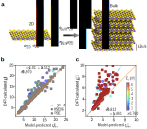
\includegraphics[width=0.95\linewidth]{img/fig4.pdf}
\caption{\label{fig-4} \textbf{Application of 2D polarizability to
    few-layer and bulk systems}.  \textbf{a-b,} Multilayer
  polarizabilities $\alpha_{\mathrm{NL}}^{\parallel}$ and
  $\alpha_{\mathrm{NL}}^{\perp}$ of selected 2D metal 
  dichacolgenides (2H-MX$_2$, M=Mo, W; X=S, Se, Te)
  as a function of number of layers $N$, respectively.  
  Inset in {\bf a,} shows a 
   scheme of the 2D-3D transition. 
  $\alpha$ in the 2D material is essentially equivalent to
  $\varepsilon$ in its bulk counterpart.  
  %
  %
  Both $\alpha_{\mathrm{NL}}^{\parallel}$
  and $\alpha_{\mathrm{NL}}^{\perp}$ linearly scales with $N$ and the
  electronic polarizability of the monolayer which indicate that
  $\alpha_{\mathrm{2D}}$ is an additive quantity under weak
  interacting regime. 
  %
  {\bf c-d,} DFT calculated $\varepsilon_{\mathrm{Bulk}}^{\parallel}$ and 
  $\varepsilon_{\mathrm{Bulk}}^{\perp}$, respectively, as a function of 
  their predicted values from the 2D polarizability model. A strong correlation 
  is observed in both components with the linear regression slope reaching the 
  unit for $\varepsilon_{\mathrm{Bulk}}^{\parallel}$ but slightly deviating for 
  $\varepsilon_{\mathrm{Bulk}}^{\perp}$ at higher magnitudes. 
  A heat map showing the dependence of $\varepsilon_{\mathrm{Bulk}}^{\parallel,\perp}$
   with the band gaps is included in {\bf d}. The model predicted values for $\varepsilon_{\mathrm{Bulk}}^{\perp}$ are in good aggreement with the DFT calculations when
  $E_{\mathrm{g}}>4$ eV. Inset in {\bf c,} shows the definition 
  of the interlayer distance in bulk $L_{\rm Bulk}$
  utilized to calculate $\varepsilon_{\mathrm{Bulk}}^{\parallel}$ and 
  $\varepsilon_{\mathrm{Bulk}}^{\perp}$ via Eqs. \ref{eq:3D-para}$-$\ref{eq:3D-para}.  %%%%  
  Calculations at the level of HSE06 and PBE are shown in circles and 
  squares, respectively, in all panels that apply. 
  }
\end{figure}






%We further look into the bulk systems. 
In a bulk material with an equilibrium
inter-layer distance $L_{\mathrm{Bulk}}$, we can follow a similar procedure as in multilayer by 
defining the polarizability as $\alpha_{\mathrm{Bulk}}$.  %of the individual layer $\alpha_{\mathrm{2D}}(L=L_{\mathrm{Bulk}})$
%
Inspired by Eqs. \ref{eq:alpha-para-def} and
\ref{eq:alpha-perp-def}, the dielectric constants
$\varepsilon^{\parallel}_{\mathrm{Bulk}}$ and
$\varepsilon^{\perp}_{\mathrm{Bulk}}$ of the bulk layered material can
be reconstructed by $\alpha_{\mathrm{Bulk}}^{\parallel}$ and
$\alpha_{\mathrm{Bulk}}^{\perp}$ as:
%
%
\begin{subequations}
\begin{align}
  \label{eq:3D-para}
  \varepsilon^{\parallel}_{\mathrm{Bulk}}
  &= 1 + \frac{\alpha_{\mathrm{Bulk}}^{\parallel}}{\varepsilon_{0} L_{\mathrm{Bulk}}}
  \approx 1 + \frac{\alpha_{\mathrm{2D}}^{\parallel}}{\varepsilon_{0} L_{\mathrm{Bulk}}} \\
  \label{eq:3D-perp}
  \varepsilon^{\perp}_{\mathrm{Bulk}}
  &= \left(1 - \frac{\alpha_{\mathrm{Bulk}}^{\perp}}{\varepsilon_{0} L_{\mathrm{Bulk}}}\right)^{-1}
  \approx \left(1 - \frac{\alpha_{\mathrm{2D}}^{\perp}}{\varepsilon_{0} L_{\mathrm{Bulk}}}\right)^{-1}
\end{align}
\end{subequations}
%
%
Here we neglect the effect of the stacking order of the layers and hypothesized 
that the basic building blocks for the dielectric response of the bulk are the polarizability of the 
individual layers subject to vdW and electrostatic interactions. 
The dielectric constant $\varepsilon$ although not well-defined for a
monolayer 2D material becomes applicable when the 2D layers are put
together as shown in the following. 
%
We compare the values of
$\varepsilon_{\mathrm{bulk}}^{\parallel}$ and
$\varepsilon_{\mathrm{bulk}}^{\perp}$ computed from DFT simulations (\textit{y}-axis)
with those predicted using Eqs \ref{eq:3D-para} and \ref{eq:3D-perp}
(\textit{x}-axis) as shown in Figure \ref{fig-4}{\textbf c} and \ref{fig-4}{\textbf d}. 
Strikingly both HSE06 and PBE datasets give almost identical results which suggest 
a non-method dependent behavior. 
%
We observe that
$\varepsilon_{\mathrm{bulk}}^{\parallel}$ values calculated by DFT and
predicted by Eq. \ref{eq:3D-para} are in sound agreement with a linear
regression slope of 1.01 and $R^2$ of 0.97. Conversely, 
$\varepsilon_{\mathrm{bulk}}^{\perp}$ values predicted from
Eq. \ref{eq:3D-perp} fairly agree with the DFT-calculated values when
$E_{\mathrm{g}}>4$ eV, while the deviation becomes larger when
$E_{\mathrm{g}}$ reduces. The above results indicate that
$\alpha^{\parallel}_{\mathrm{Bulk}}$ can generally be estimated with 
high accuracy from its 2D counterpart, while $\alpha^{\perp}_{\mathrm{Bulk}}$ differs due
to the interlayer coupling and overlap between induced
dipole\cite{Andersen_2015_dielec_vdWH,Laturia_2018}. 
Nevertheless, as most of the optical response and electronic device properties rely on the 
in-plane dielectric constant for practical applications, the possibility to handily
estimate $\alpha_{\mathrm{2D}}^{\parallel}$ from well established magnitudes of 
$\varepsilon_{\mathrm{bulk}}^{\parallel}$, for instance, from material databases,   
using reverse engineering in Eq.\ref{eq:3D-para}, it is a step forward in the 
design and understanding of the dielectric phenomena in 2D. 

%With a better model describing
%$\alpha_{\mathrm{bulk}}^{\perp}$ as function of $\alpha_{\mathrm{2D}}^{\perp}$ and
%the degree of interlayer coupling, the dielectric transition from 2D
%to 3D would be smoothly described.


\subsection{Unified geometric representation of $\alpha_{\mathrm{2D}}$}
\label{sec:unif-geom-repr}

%
Lastly, we demonstrate that both $\alpha_{\mathrm{2D}}^{\parallel}$
and $\alpha_{\mathrm{2D}}^{\perp}$ can be unified using a geometric
approach. In merit of the unit analysis,
$\alpha_{\mathrm{2D}}^{\parallel}$ and $\alpha_{\mathrm{2D}}^{\perp}$
both have unit of $4\pi\varepsilon_{0} \times$[Length]. In other words,
they represent in- and out-of-plane characteristic lengths,
respectively. 
%
It is well-known that the in-plane screened
electrostatic potential 
$V(r) = {\displaystyle \frac{e}{4 \alpha_{\mathrm{2D}}^{\parallel}}}
\left[H_{0}({\displaystyle \frac{2\varepsilon_{0}
      r}{\alpha_{\mathrm{2D}}^{\parallel}}}) - Y_{0}( {\displaystyle
    \frac{2
      \varepsilon_{0}r}{\alpha_{\mathrm{2D}}^{\parallel}}})\right]$
from a point charge as a function of distance $r$\cite{Keldysh_1979_eps_multi,Pulci_2014} 
(where $H_{0}$ is the Struve
function and $Y_{0}$ is the Bessel function of second kind) 
is associated with the in-plane screening radius
$r_{0}^{\parallel}=\alpha_{\mathrm{2D}}^{\parallel}/(2
\varepsilon_{0})$, such that $V(r,r/r^{\parallel}_{0} \gg 1)$ reduces
to the simple Coulomb potential in vacuum. Combining with the result
that $\alpha_{\mathrm{2D}}^{\perp}/\varepsilon_{0}$ characterizes the
thickness of a 2D material, we can view the dielectric screening of a
point charge sitting in the middle of a 2D material as an ellipsoid
with the radii of principal axes to be
$r_{0}^{\parallel} = \alpha_{\mathrm{2D}}^{\parallel}/(2
\varepsilon_{0})$ and
$r_{0}^{\perp} = \alpha^{\perp}_{\mathrm{2D}}/(2 \varepsilon_{0})$,
respectively, as illustrated in Figure~\ref{fig-ellip}\textbf{a}.
This is analog to the polarizability ellipsoid picture of molecules
used in spectroscopy \cite{Banwell_1994}. The polarizability ellipsoid
for a 2D material is in general ultra flat, with
$r_{0}^{\parallel} \gg r_{0}^{\perp}$, as demonstrated by layered materials 
of group 6 of 2H-TMDCs (Figure~\ref{fig-ellip}\textbf{b} and
~\ref{fig-ellip}\textbf{c}). 
%
The picture of the polarizability ellipsoid
provides further insights into the physical nature of
$\alpha_{\mathrm{2D}}$: $r_{0}^{\parallel}$ is close to the exciton
radius that it is confined within the 2D plane~\cite{Pulci_2014}. This radius is
generally larger for a smaller bandgap semiconductor, and can be
converted through the exciton binding energy as proposed in
Refs.\cite{Olsen_2016_hydrogen,Jiang_2017_Eg_Eb}.
%Eq. \ref{eq:2D-Moss-para}. 
%
$r_{0}^{\perp}$ in its turn can be 
indirectly deduced from Stark effect for perpendicular electric fields 
\cite{Pedersen_2016,Klein_2016,Roch_2018}. A comparison with 
available experimental data\cite{Verzhbitskiy19, Roch_2018} gives 
close magnitudes with our predicted values. 

Inspired by the polarizability ellipsoid model, we will show that a general 
picture of the dielectric properties in
any dimension can be drawn by studying the dielectric
anisotropy. That is, the dielectric response of a material along 
its different geometrical orientations. 
%
%
We define the dielectric anisotropy index $\eta$ as:
\begin{equation}
  \label{eq:anisotropy}
  \begin{aligned}[t]
    \eta =
    \begin{cases}
      {\displaystyle \min_{i \neq j}}
      {\displaystyle
        \left(\frac{\varepsilon^{ii}}{\varepsilon^{jj}}\right)},
      \ \mathrm{Bulk\ Materials}\\
      {\displaystyle \min_{i \neq j}}
      {\displaystyle
        \left(\frac{\alpha_{\mathrm{2D}}^{ii}}{\alpha_{\mathrm{2D}}^{jj}}\right)},
      \ \mathrm{2D\ Materials}\\
    \end{cases}
  \end{aligned}
\end{equation}
%
%
\begin{figure}[H]
  \centering
  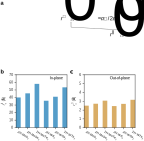
\includegraphics[width=0.8\linewidth]{img/fig-ellipsoid.pdf}
  \caption{\label{fig-ellip} \textbf{Geometric representation of the
      2D polarizability}. 
      \textbf{a,} Scheme of the polarizability
    ellipsoid of a 2D material, with its in-plane
    ($r_{0}^{\parallel}$) and out-of-plane radii
    ($r_{\mathrm{0}}^{\perp}$) proportional to
    $\alpha_{\mathrm{2D}}^{\parallel}$ and
    $\alpha_{\mathrm{2D}}^{\perp}$, respectively.  
    {\bf b-c,} Calculated magnitudes of 
    $r_{0}^{\parallel}$ and $r_{0}^{\perp}$, respectively, for selected 2D TMDCs. 
    The polarizability ellipsoid is highly anisotropic with screening much
    stronger at in-plane than out-of-plane directions. Comparison with available experimental 
    results\cite{Roch_2018,Verzhbitskiy19} for 2H-MoS$_2$ and 2H-WSe$_2$ is included.} 
\end{figure}
%
%
%
$\eta=1$ indicates that the material has isotropic dielectric properties
while $\eta \to 0$ means that the dielectric property is highly
anisotropic. Figure \ref{fig:aniso} shows the phase diagram of $\eta$
as function of $E_{\mathrm{g}}$ for 2D materials and their bulk
counterparts. Interestingly, the 2D materials (blue triangles) can be
clearly distinguished from the bulk layered materials (orange squares)
with the boundary line determined to be
$\eta =0.048 (E_{\mathrm{g}}/ \mathrm{eV})+0.087$. The much lower
$\eta$ values for 2D materials compared with their bulk counterparts
indicates a high dielectric anisotropy, which is responsible for the
unique 2D optoelectronic properties, such as the electrostatic
transparency phenomena\cite{Liluhua_2014,Tian_2016,Li_2018} and the large exciton
binding energies
\cite{Pulci_2014,Tran_2014,Chernikov_2014_EB_MoS2_2D3D,Berkelbach_2013}. From
Eqs. \ref{eq:2D-Moss-para}, \ref{eq:2D-Moss-perp} and
\ref{eq:anisotropy} we can see $\eta$ is roughly proportional to
$E_{\mathrm{g}} \times \delta$, which explains the observation that
$\eta$ for 2D materials increase almost linearly with
$E_{\mathrm{g}}$, since the layer thickness $\delta$ (mostly 3--10
\AA{}) of the 2D materials investigated varies much less than
$E_{\mathrm{g}}$ in the range of 0.1--7 eV (Figure \ref{fig-3}b$-$\ref{fig-3}c). 
Further analysis shows that the dielectric anisotropy
index of any bulk layered material $\eta_{\mathrm{Bulk}}$ obeys
$\eta_{\mathrm{Bulk}} \geq {\displaystyle \frac{4
    \eta_{\mathrm{2D}}}{(\eta_{\mathrm{2D}}+1)^{2}}} \geq
\eta_{\mathrm{2D}}$, where $\eta_{\mathrm{2D}}$ is the anisotropy
index of corresponding 2D layer, which is the basis for the
separation of bulk and 2D regimes in the $\eta-E_{\mathrm{g}}$ phase
diagram (Supplementary Section \ref{SI-sec:aniso}).  
%
For comparison, we also superimpose the dielectric
anisotropy indices of common semiconducting materials in other
dimensions on
the phase diagram in Figure \ref{fig:aniso}. Bulk covalent 3D (e.g. Si, GaN) and 0D (e.g. fullerenes) semiconductors show isotropic
dielectric properties, scattered along the line $\eta=1$. 
%
Conversely, reduced dimensionality increases the dielectric anisotropy of
materials such as planar organic semiconductor (OSc) in 1D-2D 
(e.g. CuPc), carbon nanotube (CNT) in 1D, linear OSc in 0D-1D
(e.g. polyacene and polyacetylene). 
%
Interestingly, most of these
materials also scatter along the boundary line separating the bulk and
2D regimes, indicating that the criteria distinguishing 2D (more 
anisotropic) and bulk materials (more isotropic) from the
$\eta-E_{\mathrm{g}}$ diagram, can also be applied to other
dimensions. From the phase diagram, we can see that 2D and bulk
layered materials, including 2D van der Waals heterostructure
(vdWH)\cite{Novoselov_2016}, provides more flexibility in
controlling the dielectric and electronic properties, compared with
covalent semiconductors (without vdW gaps) in other dimensions.


\begin{figure}[H]
  \centering
  \includegraphics[width=1.01\linewidth]{img/fig5.pdf}
  \caption{\textbf{Phase diagram of dielectric anisotropy $\eta$ as
      function of bandgap $E_{\mathrm{g}}$}. The
    $\eta$-$E_{\mathrm{g}}$ values of 2D materials (blue triangle) and
    their bulk counterparts (orange square) can be distinguished by
    the line $\eta=0.048(E_{\mathrm{g}}/\mathrm{eV})+0.087$. $\eta-E_{\mathrm{g}}$ values of
    semiconducting materials in other dimensions are also superimposed
    for comparison. Isotropic dielectric property is observed for bulk
    covalent materials (3D, red triangle) and fullerenes (0D, green
    star), while reduced dimensional materials, including planar
    organic semiconductor(OSc, 1D-2D, brown triangle), carbon nanotube
    (CNT, magenta circle) and linear OSc (0D-1D, violet pentagon) are
    scattered along the boundary line. The dimensionality and
    structure of typical materials are shown along the axis on the
    right. Compared with other materials, 2D materials and their bulk
    counterparts provide more flexibility of controlling the
    dielectric anisotropy.}
  \label{fig:aniso}
\end{figure}



\section{Conclusion}
%\label{sec:org5fd1f1a}
%\todo[inline]{To be changed later when everything fixed}

Our results show that the 2D electronic polarizability
$\alpha_{\mathrm{2D}}$ is a local variable determining the dielectric
properties of 2D materials.  There exist well-defined relationships
between $\alpha_{\mathrm{2D}}$ and other quantities hidden in the
electronic properties.  According to our analysis, simple scaling
equations involving bandgap and layer thickness can be used to
describe both dielectric and electronic features at the same
footing. A dielectric anisotropy index is found relating any material
dimension with its controllability.  Thus, our results suggest that
the challenge of understanding the dielectric phenomena is in general
a geometrical problem mediated by the bandgap. We believe the
principles presented here will benefit both fundamental understanding
of 2D materials as well as a rational device design and optimization.




\section{Theoretical Methods}
\label{sec:org8457dbb}

Simulations were carried out using plane-wave density functional
theory package VASP \cite{Kresse_1993,Kresse_1996_1,Kresse_1996_2}
using the projector augmented wave (PAW) approach with GW
pseudopotentials \cite{Kresse_1999_pseudopotentials}. Band gaps were
calculated using the Heyd-Scuseria-Ernzerhof hybrid functional (HSE06)
\cite{Heyd_2003,HSE_2006}, with spin orbit coupling (SOC) explicitly
included. The geometries were converged both in cell parameters and
ionic positions, with forces below 0.04 eV/\AA. To ensure the accuracy
of dielectric property of monolayer, a vacuum spacing of $>$ 15 \AA~is
used. A k-point grid of \(7\times7\times1\) was used to relax the
superlattice, with an initial relaxation carried out at the
Perdew-Burke-Ernzerhof
(PBE)\cite{Perdew_1996,Ernzerhof99,Paier_2005_PBE}
exchange-correlation functional level and a subsequent relaxation
carried out at HSE06 level, allowing both cell parameters and ionic
positions to relax each time. In VASP, the tag PREC=High was used,
giving a plane wave kinetic energy cutoff of 30\% greater than the
highest given in the pseudopotentials used in each material. This
guarantees that absolute energies were converged to a few meV and the
stress tensor to within 0.01 kBar.  Calculation of the macroscopic
ion-clamped dielectric tensor were carried out with an
18$\times$18$\times$1 k-grid and electric field strength of 0.001
eV/\AA.  Local field effect corrections are included at the
exchange-correlation potential $V_{\mathrm{xc}}$ at both PBE and HSE06
levels. The materials from Ref.\citenum{Haastrup_2018} for comparison
were choses with the GW bandgap larger than 0.05 eV. Bulk layered
materials were constructed by relaxing the c-axis length of
corresponding monolayer material with the interlayer van der Waals
(vdW) interactions calculated by non-local vdW correlation
functional\cite{Lee_2010_vdFD2}.  The dielectric properties of bulk
layered materials using VASP were calculated at HSE06 level with
18$\times$18$\times$6 k-grid with same parameter as for monolayer,
while the dielectric properties of bulk counterparts of
Ref.~\citenum{Haastrup_2018} are calculated at PBE level with a
k-point density of 10~\AA$^{-1}$. Local field effect corrections are
also used for the dielectric properties of bulk systems.



\section*{Data Availability}
The data that support the findings of this study 
is available within the paper and its Supplementary Information.  

\subsubsection*{Competing interests}
The Authors declare no conflict of interests.


\subsubsection*{Acknowledgments}
C.J.S. and T.T. are grateful for financial support from ETH startup funding. 
L.H.L. thanks the financial support from Australian Research Council (ARC) 
via Discovery Early Career Researcher Award (DE160100796). 
E.J.G.S. acknowledges the use of computational resources from the UK 
Materials and Molecular Modelling Hub for access to THOMAS 
supercluster, which is partially funded by EPSRC (EP/P020194/1); and CIRRUS Tier-2 HPC 
Service (ec019 Cirrus Project) at EPCC (http://www.cirrus.ac.uk) funded 
by the University of Edinburgh and EPSRC (EP/P020267/1). 
The Department for the Economy (USI 097) is acknowledged for funding support.  


\subsubsection*{Author Contributions}
E.J.G.S. conceived the idea and supervised the project. 
T.T., D.S., D.H. and E.J.G.S. performed the first-principles simulations 
and data analytics. T.T. developed the analytical model with 
inputs from E.J.G.S. and C.J.S. L.H.L. and J.N.C. 
performed numerical analysis and contributed to the discussions together with M.C.
E.J.G.S. and T.T. co-wrote the manuscript with inputs from all authors. 
All authors contributed to this work, read the manuscript, discussed 
the results, and all agree to the contents of the manuscript. 


\section*{Supporting Information}

The Supporting Information contains detailed descriptions and
discussions about dielectric properties of 2D materials, effective
dielectric model, derivations of the 2D polarizability-based model,
dependency of $\alpha_{\mathrm{2D}}$ on the choice of bandgap,
relation between 2D and 3D properties, explanations of the dielectric
anisotropy, as well as raw data sheet from first principles
calculations. 



\bibliography{ref}

% \section{Figures}
\label{sec:org34cbe74}
\clearpage

\section*{TOC entry}
\begin{figure}
  \centering
  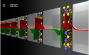
\includegraphics[width=0.95\linewidth]{img/toc.pdf}  %toc.pdf  
\end{figure}


\end{document}
%%% Local Variables:
%%% mode: latex
%%% TeX-master: t
%%% End:
